\chapter{Saving Millions in Government Procurement Through Data Science and Market Design}

\section{Introduction}


When conducting their procurement processes, large organizations can choose among different mechanisms to select their supplier base. With a centralized approach, the organization may choose to run an auction to select a single supplier. By contrast, with a decentralized approach, the purchasing decisions are made by the different suborganizations or units, which may run their own auctions or buy the products they need in the open market. Although there is an increasing trend to centralize purchases through central procurement bodies (see,  e.g., \cite{oecd2019reforming}) there are pros and cons to procurement centralization. On the one hand, centralization may allow for tighter control of expenditures and may be able to take advantage of the economies of scale and purchasing power resulting from aggregating the demand of the different buying units. On the other hand, decentralization may be advantageous when the purchasing units have heterogeneous needs and local information on the supplier base and on the market dynamics, which may lead to more efficient procurement \citep{dimitri2006handbook}.

Framework agreements (FAs)  provide an intermediate approach between centralization and decentralization of purchases. In a FA, a central procurement agency pre-selects an assortment of products and suppliers that remains valid for a given time horizon. Then, each affiliated organization can purchase from this selected assortment as needed. Examples of such mechanisms include the purchase of computers in a university and health plans with lists of prescription drugs available to plan enrollees, among others. Due to their flexibility, FAs are nowadays  recognized as a fundamental tool in public procurement \citep{albano2016law}. {As an example, our collaborator, the Chilean government central procurement agency (Direcci\'on ChileCompra, or ChileCompra for short) purchased US\$3,000,000,000 worth of goods and services though FAs in 2018, which represented 22.6\% of the value of all public procurement in Chile} \citep{datosabiertos}.%\todoMO{Updated number and ref}

In government FAs, the pre-selection of suppliers is usually conducted through a first-price auction {per product} where bids correspond to the selling prices of the suppliers added to the FA. Once selected, the FA assortment of suppliers and products is usually available for multiple years, allowing government organizations to purchase as needed. Moreover, the bids in the auction effectively act as ceiling prices: while the FA is in place, the suppliers are allowed to decrease their prices through promotions or price changes, but price increases are heavily regulated and are mostly governed by inflation.

In designing the FA auction rules, the central procurement agency must consider the induced price competition among suppliers to optimize the following trade-off. On the one hand, rules for which only a few {products} {suppliers per product} end up being in the FA (more competitive auction rules) may increase suppliers' incentives to place aggressive bids in the auction, so that {their products} {they} have a better chance of being part of the small selection of items. Thus, this will result in lower ceiling prices. On the other hand, rules for which it is “easy” to be part of the FA (less competitive rules) may result in higher bids and hence higher ceiling prices. At the same time, they will result in more suppliers being added and thus, potentially, in more intense price competition and more promotions during the FA which may result in lower purchasing prices. As the government ultimately cares about spending (and hence the prices at which transactions occur), a natural question is whether more competition in the FA auction will effectively reduce government spending.

In theoretical work, \cite{saban2021procurement} (see also the follow-up paper, \cite{Choi22}) study these sources of competition in stylized models of FAs and show that increasing competition in the auction stage  typically reduces  spending. %prices and improves market outcomes. 
Specifically, they show that bids under less competitive auctions are significantly higher than those under more competitive  rules, even if suppliers account for price competition during the FA. That is, price competition inside the FA does not compensate for the lower prices obtained by using more competitive auctions. Indeed, the motivation for this theoretical research stemmed from our initial exploratory analysis of ChileCompra FAs, aiming at enhancing our understanding of them. Subsequently, showcasing our findings to the ChileCompra executives led to the applied project documented in this paper. 
Specifically, \textit{this paper reports on a market design intervention in which we redesign a large FA run by the Chilean government to understand the effects of increasing competition at the FA  auction}. We show that this change indeed resulted in important savings for the government.
Thus, our efforts have come full circle: from the practical application to a theoretical exploration and back to the application.


%\ds{Broadly speaking, these papers show that the bids under less competitive auctions are significantly higher than those under more competitive auction rules, even if suppliers account for the fact that they may need to lower their prices once in the FA and, moreover, the price competition inside the FA will not be as aggressive as to offset the lower ceiling prices that can be obtained by using more competitive auctions.
%}


As a first step, we performed an initial descriptive analysis of ChileCompra's 2014 Food FA, used by the Chilean government between 2014 and 2017 to purchase US\$200 million worth of products annually. This analysis revealed low levels of competition at the auctions used to define the FA assortment. For instance, about half of the auctions in the FA received a single bid and {84\%} of all bids were awarded. The high number of auctions with a single bid may be explained by the fact that suppliers self-reported their product attributes using free unstructured text, which resulted in identical products being treated as different ones and thus not being part of the same auction. As stated above, the bids in these auctions act as ceiling prices; thus, this observed low competition in the auction may have resulted in higher ceiling prices and, potentially, in higher transaction prices. At the same time, using data from the operation stage of the 2014 Food FA, we observed that the prices at which products were sold tend to be below the bid price, revealing some competition in the operation stage to attract demand.
%Because the bids in these auctions act as ceiling prices once in the operation stage, low competition in the bidding stage could induce high posted  and transaction prices in the marketplace.

With this motivation, we collaborated with Chilecompra to redesign the 2017 Food FA. The new design consisted of two main changes. First, we built Natural Language Processing (NLP) algorithms to standardize the catalogue of products that would be required in the auction stage, defining each product based on objective attributes. This standardization was useful to: (i) analyze government purchases in the FA 2014 and identify the products to be included in the new 2017 FA based on their observed demand; (ii) define the specific characteristics of the products that suppliers would bid in the auction stage. Altogether, defining a structured catalogue was fundamental to build a comprehensive assortment of products that would cover government needs; with this innovation, suppliers were not allowed to self-report additional products to be offered, which as described earlier, could lead to reduced competition in the auctions.

The second main change in the new FA took advantage of the catalogue standardization to implement an experimental design to evaluate whether introducing more intense competition in the auction stage could lead to lower prices in the marketplace. This randomized field experiment assigned product categories to different thresholds to award the winning bids: products in the control group awarded the lowest 80\% of the bids -- a low competition scenario similar to what was awarded in the FA 2014. In contrast, products in the ``high competition'' treatment had a stringent threshold, awarding to only the lowest 20\% of bids.


We measured the impact of this intervention on submitted bids, winning bids, the prices that were posted in the ChileCompra marketplace, and the transaction prices, using a difference-in-differences estimation approach that matched products between the old and new auction designs. The empirical results show that products that were in the 20\%  treatment in the auction stage had 8.1\% lower awarded median bids, and 8.2\% lower transacted median prices. Savings in the procurement cost of the government amounted to US\$3.6 million  yearly  in the treatment group and to US\$11 million yearly if we extrapolate them to the entire Food FA.

After the successful implementation in the Food FA, ChileCompra started to implement a similar design in all of its FAs, and many of these improvements were included in the new regulation on government purchases \citep{leycompras}. By 2022, most of the operating FAs had adopted the new design    (\cite{cuentapublica2021},\cite{datosabiertos}).
Similar to the Food FA, these new FAs incorporated a structured product catalogue (with the assistance of automated algorithms to structure product attributes) and enforced tighter competition to enter the FA using lower thresholds to award bids. ChileCompra executives reported successful implementations and if we extrapolate the savings from the Food FA to all the FAs operating in 2022, the total savings amount to around US\$64 million per year.%\todoMO{Updated number}

 Overall, our work shows the value of restricting competition in the FA auction, providing important guidelines on how to implement FAs in practice. Furthermore, our work contributes to the literature on applied market design in which  theory and algorithms, together with a deep understanding of the institutional and operational details of the market are used to improve outcomes \citep{vulkan2013handbook}.

\section{Background: Framework Agreements in Chile's Public Procurement System}

In this section we briefly describe FAs. Then, we describe in detail the auction stage and its potential problems of the FA run by ChileCompra in 2014 to source food products to the public organizations in Chile. This FA operated from November 2014 to August 2018 and we refer to it as the 2014 Food FA or simply FA 2014.



%\input{FAs_and_problems_revision}

% Veriricar fechas del auction (cuando reciben bids, cuando adjudica, etc).

A {\bf framework agreement (FA)} is a purchasing mechanism by which a central procurement agency (in our case, ChileCompra) selects a set of suppliers and agrees on the terms and conditions that will be applied to any subsequent transaction over a pre-specicfied time horizon.
At a high level, an FA can be thought of as a process consisting of two main stages: an auction stage and an operation stage. %\ds{stages? phases?}

%\ds{[Add graph]}

%\ds{public tender -> auction. Also need to agree on verb tenses (past, future, presemt) }
In the \emph{auction stage}, the central procurement agency publishes the rules of the auction, including which products they are seeking to purchase and the rules to decide which suppliers and products will be offered as part of the FA. {Hence, this first stage of the FA runs multiple independent simultaneous auctions, one for each product. Each auction determines a set of suppliers for a single product, with suppliers submitting bids that include price and additional details, which we explain below.} Using the published rules, ChileCompra determines the supplier--product combinations added to the FA, i.e., added to ChileCompra's online marketplace. The awarding rules may vary across FAs and includes a combination of price and quality certifications. This concludes the auction stage. 

In the \emph{operation stage} the awarded suppliers offer their products in an electronic procurement marketplace operated by ChileCompra. Buyers from public organizations can use this marketplace to purchase products directly from the suppliers' assortment selected in the FA auction stage, without running an additional tendering process. This allows public organizations to purchase goods according to their preferences and in an agile way, speeding up buying. In the case of ChileCompra, the FAs implemented before 2018 lasted for about four years.  During the operation, suppliers can make discounts to the bid prices submitted in the auction stage; consequently, the auction price becomes a \textit{ceiling price} during the operation stage.


\subsection{Description of the 2014 Food Framework Agreement}\label{sec:FA2014}

% 1.- Catálogo y estructura de productos
% 2.- Cómo se define una oferta
% 3.- Resultados
% 4.- Resumen de problemas del Convenio.

\noindent{\bf FA definition.}
In 2014, ChileCompra carried out an auction for the FA of perishable and non-perishable foods. Within food items, ChileCompra defined a preliminary list of products of interest, and potential suppliers were invited to submit bids for these products. Each product comprised three attributes defined by ChileCompra: category (e.g., drinks), type of product (e.g., juice), and brand (e.g., Andina). Potential suppliers were allowed to submit bids for \emph{any} product matching these attributes. We describe the rules that decided the winning bids below. {After the winning bids were selected, the FA was expected to be in operation for three years.} 

\noindent {\bf Bidding process.}
To submit a bid for a product, potential suppliers had to provide two additional attributes: model (e.g., orange 250 ml.) and units (e.g., 4 bottles). A key aspect here is that the definition of these two attributes by the suppliers in the bidding process was done using free unstructured text.  Once a product was defined with the five attributes (three defined by Chilecompra and two by the bidder) suppliers had to provide a price; this price will effectively act as a ceiling price during the operation of the FA.\footnote{As we later discuss, suppliers are allowed to decrease the price during the operation phase of an FA; by contrast, price increases are heavily regulated and can, for the most part, only be adjusted for inflation as dictated by the national inflation index.} 
Suppliers were required to also provide general selling information, including compliance with regulations and shipping rates for the different regions, among others. In addition to the bids for products included in Chilecompra's catalogue, each seller could choose to submit bids for up to 60 \emph{new} products (which also include five attributes in their specification).  The auction rules were defined differently depending on whether the product was perishable or nonperishable. For nonperishable products, all bids submitted for the same product -- defined by its five attributes -- competed in the same auction. For perishable products, suppliers competed only with other suppliers located in their same geographic region.


% \input{tables/bids_description/table_2014_bids_results}

%\ds{discuss table. SKUs defined by Chilecompra has 2 attributes that are defined by suppliers. Explain this in tables note. Also, explain what is a rejected SKU. Add \% of bids awarded per auction.}

 
  
  \noindent {\bf Awarding the set of suppliers.} A supplier's bid was assessed according to a weighted sum of scores associated with five dimensions, including price, technical requirements, sustainability characteristics, shipping costs, and volume discounts. Each dimension score was normalized to a 0--100 scale. The score for price was computed relative to the minimum bid price among all bidders in the auction (excluding extreme outliers), and received a 60\% weight in the final score. Scores for the shipping costs and volume discounts were also computed relative to minimum bids among all suppliers, whereas sustainability and technical requirements were calculated based on specific criteria that do not depend on the others' bids. In terms of the weight for the final score, regional shipping costs accounted for 15\%, volume discounts for 20\%, sustainability for 3\%, and technical requirements for 2\%. For more details on the score calculations, see \cite{levy2017rediseno}. All bids with a total score above 70 points were awarded. In addition, if a supplier was awarded 80\% or more of the bids, all of its bids were awarded.

%\input{tables/bids_description/table_2014_awd_score}
%\input{tables/bids_description/table_2014_price_score}

%\ds{discuss tables? Discuss perishable vs non-perisable. Discuss focusing on pantry.}

\subsection{{Analyzing competition in the 2014 Food FA} }  \label{se:noncomp}

We collected bid data for the 2014 Food FA auction, which is summarized in Table \ref{tab:bid_results_2014b}. {Of the 10,664 auctions that were awarded,  47.3\% received only one bid, with no competition upon entry. Overall, about 84\% of submitted bids were awarded, suggesting low competition to enter the market (recall that the awarding criteria can include multiple awarded bids per auction). The lack of competition was particularly severe for products where suppliers defined the product attributes, leading to 93.8\% of these auctions receiving a single bid and 1.1 bids per auction on average. Bids for the  auctions in which suppliers defined {all} product attributes had a 99.7\% of winning, with essentially no competition whatsoever. These findings are consistent to those presented in the study by  \cite{oecd2017Chile} for other FAs. The absence of standardized product definitions, low selectivity in the awarding process, coupled with suppliers strategically differentiating  their products to sidestep competition during the auction stage,  resulted in this noticeable lack of competitive forces.}


%, presenting Chile's FA system as relatively open marketplace prioritizing inclusion over competition.\ds{no se si ayuda}


\begin{table}[t]
\caption{\label{tab:bid_results_2014b}{Summary of the  2014 Food FA auction stage}}
\centering
\resizebox{\textwidth}{!}{
\begin{threeparttable}
\begin{tabular}[t]{lcccc}
\toprule
  & \# Auctions & Avg. \# bids & \% Awarded Bids & \# Single bid Auction\\
\midrule
All products & 10664 (100.0\%) & 3.7 & 83.9 & 5046 (47.3\%)\\
Defined by ChileCompra & 8765 (82.2\%) & 4.2 & 80.5 & 3265 (37.3\%)\\
Defined by suppliers & 1899 (17.8\%) & 1.1 & 99.7 & 1781 (93.8\%)\\
\bottomrule
\multicolumn{5}{l}{\textsuperscript{} }\\
\end{tabular}
\begin{tablenotes}
\small
\item \textit{Notes}: {Products labeled ``Defined by ChileCompra" include those where the first three attributes were fixed by Chilecompra and two other attributes by the supplier. ``Defined by suppliers" indicate those products where suppliers defined all five attributes. {For each segment (``All products,'' ``Defined by ChileCompra,'' ``Defined by suppliers''):  ``\# Auctions" counts the number of separate auctions that were ran in that segment; ``Avg. \#  bids" is the average number of bids per auction; ``\% Awarded Bids" is the fraction of submitted bids that were awarded; and ``\# Single-bid Auctions" is the number  of auctions with  only one bid  submitted.} }
    \end{tablenotes}
\end{threeparttable}}
\end{table}

%\input{tables/bids_description/table_fa_2014_merged}


At first glance, this lack of competition may appear to be worrisome. For instance, a common finding in the auction design literature (see, e.g., \cite{myerson1981optimal, klemperer2004auctions}) is that, in general, attracting more bidders to the auction will decrease bids and hence purchasing prices. However, this finding applies to standard auctions, but may not apply to framework agreements {that have a subsequent operation stage}. To see why, we next explain the different dimensions of price competition in FAs.

\noindent{\bf Price competition in the FAs.}
Broadly speaking, there are two different ways in which suppliers may compete in prices during a FA (see also \cite{Demsetz68}). The first mechanism is \textit{competition in the auction stage to enter the FA}. In general,  whether a supplier is included  in the FA depends on the rules of the auction and the bids placed by it and the other suppliers participating in the same auction. By placing a lower bid, a supplier typically increases its chances of being part of the FA. Obtaining low bids may be important as bids effectively act as ceiling prices. Therefore, more competitive auctions may lead to lower bids and, potentially, to lower transaction prices. 

The second mechanism is \textit{price competition in the operation stage to attract demand.} An important characteristic of an FA relative to other more commonly used auction mechanisms is that, even when a supplier is added to the FA, it is not guaranteed any fixed number of orders. In fact, there is competition within the FA assortment between all the suppliers offering similar products to capture the demand for those products. \textit{Suppliers are allowed to lower the prices of their products once in the FA}, either temporarily via promotions or permanently by requesting a price change. Naturally, one would expect that by lowering their prices, suppliers may be able to increase their market share.  As a result, suppliers may also compete in prices during the operation stage of the FA.
{This may be more apparent when one considers the long time horizon of a FA and that the most cost-efficient suppliers may change over time. In this situation, more competition in the operation stage may induce cheaper suppliers to decrease their mark-ups through promotions throughout the FA  in order to price out competitors. This type of competition is not captured by the initial auction ceiling prices.}

{Table \ref{tab:FA2014_cat_wPrice} provides examples that illustrate competition in the auction and operation phase. Each row corresponds to a different auction for a specific product, where suppliers submitted bids to enter the market. The product description provides the characterization of the product to be offered, which was specified as free text. To better understand the characteristics of these products, we added the columns Subcat, Type, Brand, Format and Units which describe attributes of the products (to be clear, these attributes \textit{were not} included in the products specifications of the FA 2014 -- we added them to better explain the similarity across products). These examples reveal that several products had  similar characteristics but were assigned to different auctions. For example, the same product sold in packs of 10 and 25 units were considered to be different and ran on separate auctions. Furthermore, for the ``spaghetti 87'' product, a pack of 5 units of 1 kg. was considered to be different from the same product sold in one unit of 5 kgs.}


{The Bid price column in the table describes the average bid submitted by the awarded suppliers for each auction (normalized per unit, to facilitate the comparison across different pack sizes). Recall that awarded suppliers are not guaranteed demand: they have to attract buyers during the operation stage and are allowed to lower prices below the bid price. Hence, {it is quite possible that similar products could face competition during the operation stage even as they were awarded on separate auctions.} To see this, we collected data from the operation stage of the FA 2014 to calculate the prices at which these products were actually sold in the marketplace. These data show that selling prices are below the bid price, revealing  competition in the operation stage to attract demand for these particular products.}

\begin{table}[H]\caption{Examples of auctions in the  FA 2014 including the full description of the auctioned product, which was partially entered by  the suppliers using unstructured text.}
\scriptsize{
    \resizebox{\textwidth}{!}{
    \begin{tabular}{lllllllllll}
    \toprule
    Auction & Full Product Descriprion 
    & Subcat & Type                        & Brand       & Format    & Units &  Bid price & Transaction Price \\
    \midrule
    966390  & agua mineral benedictino con gas 500 cc 6 unidades   & water  & sparkling mineral water     & Benedectino & 500 ml.   & 6      & 384.8     & 276.1             \\
    966395  & agua mineral benedictino con gas 500 cc unidad       & water  & sparkling mineral water     & Benedectino & 500 ml.   & 1      & 388.7     & 288.7             \\
    966634  & agua mineral ccu con gas cachantun 2,25 l 6 unidades & water  & sparkling mineral water     & CCU         & 2,250 ml. & 6      & 550.8     & 453.7             \\
    966677  & agua mineral ccu con gas cachantun 2,25 l unidad     & water  & sparkling mineral water     & CCU         & 2,250 ml. & 1      & 576.5     & 423.2             \\
    966640  & agua mineral ccu sin gas cachantun 1,6 l 6 unidades  & water  & non-sparkling mineral water & CCU         & 1,600 ml. & 6      & 459.6     & 394.8             \\
    966683  & agua mineral ccu sin gas cachantun 1,6 l unidad      & water  & non-sparkling mineral water & CCU         & 1,600 ml. & 1      & 467.1     & 396.3             \\
    966642  & agua mineral ccu sin gas cachantun 500 cc 6 unidades & water  & non-sparkling mineral water & CCU         & 500 ml.   & 6      & 349.3     & 269.9             \\
    966685  & agua mineral ccu sin gas cachantun 500 cc unidad     & water  & non-sparkling mineral water & CCU         & 500 ml.   & 1      & 347       & 224.3             \\
    \midrule 
    966580  & pasta carozzi spaghetti 3 400 gr 10 units            & pasta  & spaghetti                   & carozzi     & 400 gr.   & 10     & 465.2     & 380.3             \\
    966595  & pasta carozzi spaghetti 3 400 gr 25 unidades         & pasta  & spaghetti                   & carozzi     & 400 gr.   & 25     & 467.3     & 422.9             \\
    966615  & pasta carozzi tallarin 87 1 k 5 unidades             & pasta  & spaghetti                   & carozzi     & 1,000 gr. & 5      & 1230.7    & 1065.9            \\
    966582  & pasta carozzi tallarin 87 400 gr 10 unidades         & pasta  & spaghetti                   & carozzi     & 400 gr.   & 10     & 462.9     & 429.2             \\
    966598  & pasta carozzi tallarin 87 400 gr 25 unidades         & pasta  & spaghetti                   & carozzi     & 400 gr.   & 25     & 473.6     & 405.7             \\
    966622  & pasta carozzi tallarin 87 5 k unidad                 & pasta  & spaghetti                   & carozzi     & 5,000 gr. & 1      & 5303.4    & 3956.1  \\ 
    \bottomrule
    \end{tabular} }

}
    \small{ \textit{Notes:} The columns subcat(egory), type, brand, format, and units were coded manually and were not specified in the 2014 Food FA. The format describes the weight/volume of each unit, and ``\# Units'' describes how many units are included in a pack. Bid and transaction prices are calculated as the averages across all awarded suppliers, normalized per unit and adjusted using the Food CPI.}
    \label{tab:FA2014_cat_wPrice}
\end{table}


The lack of standardization leads to high redundancy of the products offered in the marketplace, in which approximately 40\% of the awarded products were not sold during the operation stage and, in fact, 50\% of the products with lowest sales volumes only represented 1\% of total purchases.  Moreover, because suppliers were also allowed to add products during the operation stage of the FA, the lack of product standardization made it very hard for Chilecompra to check if these ``new'' products were already offered in the marketplace, further exacerbating the redundancy in variety. In fact, a visual inspection of the products added during the operation of FA 2014  revealed that many of them corresponded to products that were already  part of the assortment.

To further illustrate the consequences of allowing suppliers to define their own products using free text, Figure \ref{fig:nescafe} illustrates an example for the ``Nescafe" instant coffee brand. The image shows 6 products, 4 of them are identical and a fifth one is very similar (with a small increase in the grams). Although the products are the same, they did not compete in the auction stage: suppliers were effectively entering them as different products in their bids or adding them as new products during the operation stage. In section \ref{sec:designFA}, we provide further evidence that this redundancy in product variety is systematic across products in the FA 2014. 

\begin{figure}
    \centering
    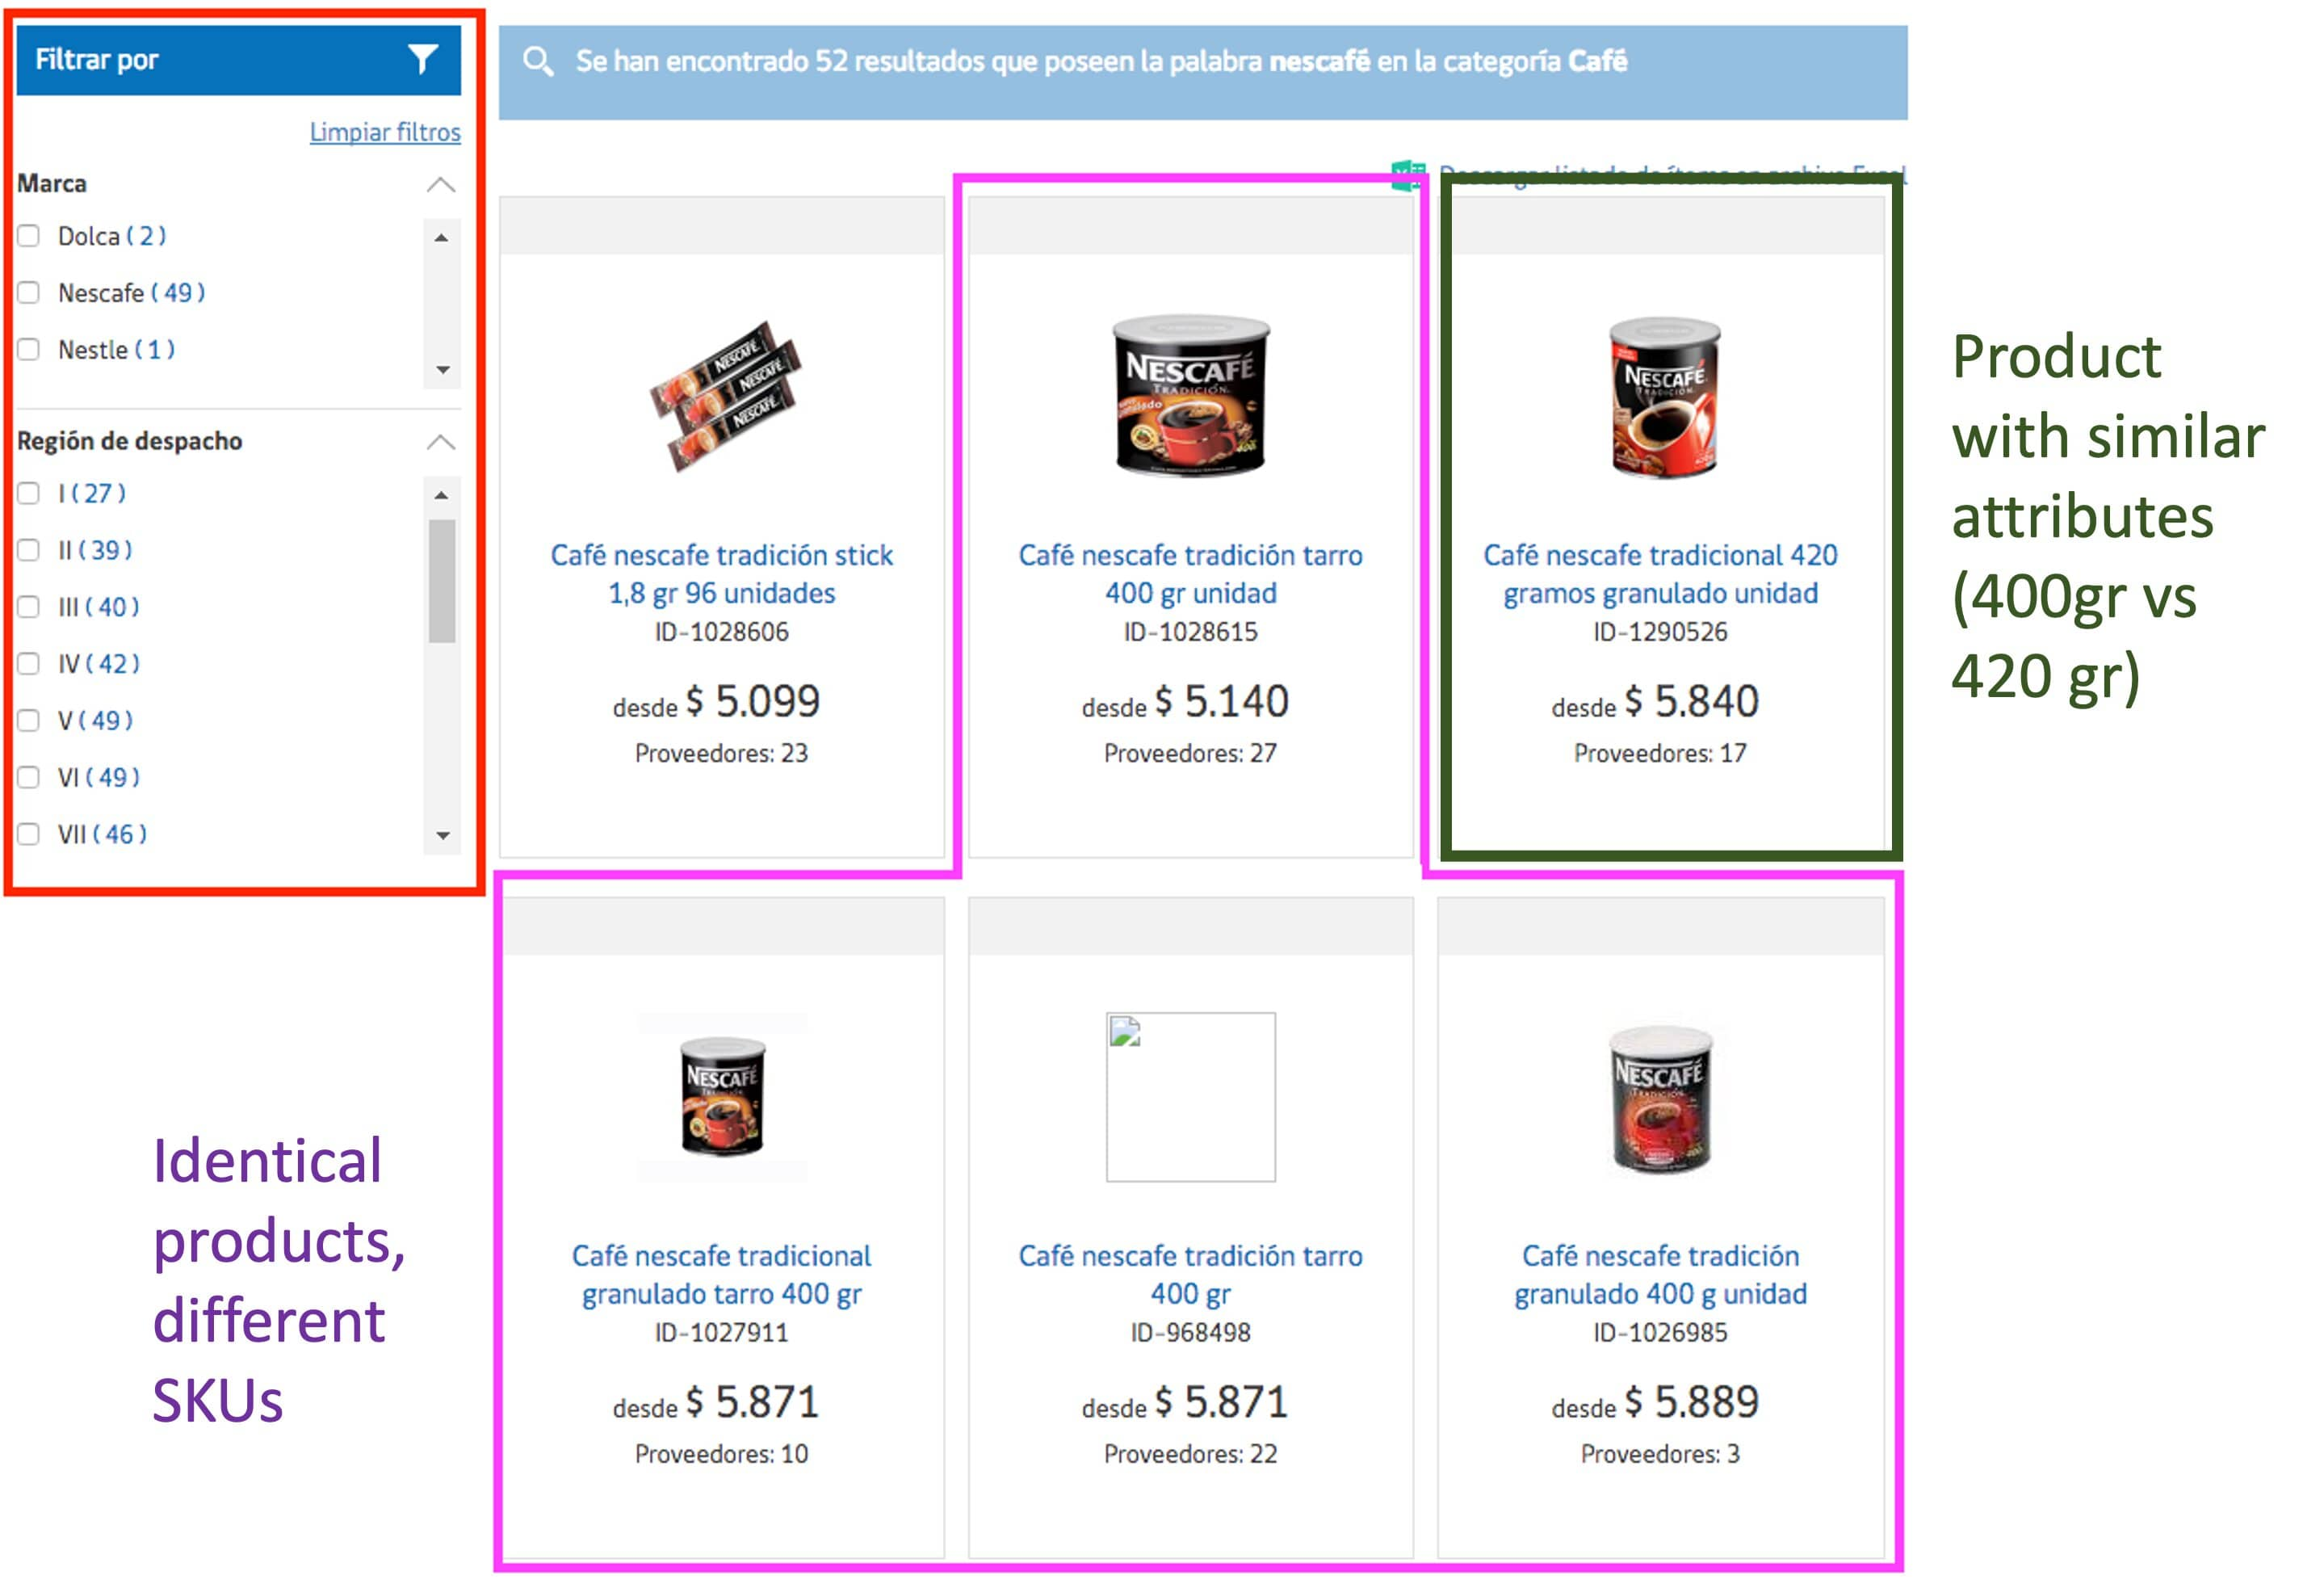
\includegraphics[scale=0.6]{imagenes/procurement/nescafe example.jpg}
    \caption{Example of similar products offered in the operation stage of the FA 2014. The search ``Nescafe'' displays multiple products corresponding to this instant coffee brands. Four products are identical and another one is very similar (with a small variation in the size). None of these products competed among them in the auction stage: they where either considered in separate auctions or added by suppliers as new products during the operation stage. }
    \label{fig:nescafe}
\end{figure}

\noindent{\bf Should FA auctions be more competitive?} Based on the above discussion, it is unclear whether making the rules of the auction more competitive translates to lower government spending. On the one hand, it is true that by making the auctions more competitive, the auctioneer may be able to decrease the awarded bids and hence the ceiling prices. On the other hand, if fewer bids are awarded, then there will be fewer suppliers in the FA, which in turn may decrease the price competition during the operation of the FA. 

{A series of papers employing mechanism design and auction models with incomplete information have been published with the intent of elucidating the aforementioned trade-off. Specifically, \cite{saban2021procurement} and its subsequent paper \cite{Choi22} present stylized models of FAs, primarily focusing on understanding the impact of increasing auction competitiveness by limiting entry into the FA. Their findings indicate that limiting entry into the FA can indeed lead to reduced purchasing prices. This observation is valid even in scenarios where suppliers behave strategically, recognizing that while they might not compete for entry into the FA, they will face competition within the FA to attract demand.}\footnote{{An important simplification in these studies is the assumption that suppliers set a single price, which serves a dual purpose: competing in the FA auction and within the FA itself. This stands in contrast to the more realistic scenario where a ceiling price is set during the auction, with potential discounts applied within the FA. Regardless of this simplification, the models effectively highlight the primary effects of introducing competition into the auction.}}


To shed light on this market design question in a real-world setting, we worked in collaboration with ChileCompra in the design of a new Food FA, where we tested the impact of increasing competition in the auction stage of the FA on public spending. We describe this initiative in the next section.

%\ds{discuss lo que viene.}


%Recall that bid prices to enter the market constitute a ceiling price, allowing suppliers to also compete within the market. Hence, low competition to enter the FA may still lead to low transaction prices if the price competition during the operation of the FA is intense. 



%To shed light on this market design question, we worked in collaboration with ChileCompra in the design of a new food FA, in which we standardize the product catalogue and also tested the impact on public spending of increasing competition to enter the market. We describe this initiative in the next section.

%\input{tables/bids_description/table_competition_fa_2014}


 

% \begin{figure}[H]
% \centering
% \label{fig:operation_fa}
% \includegraphics[scale=.5]{figures/plot_p.bids2014_both.pdf}
% \caption{Number of auctions of Pantry Products by percentage of awarded bids. This distribution excludes auctions in which the total number of bids were awarded.}
% \end{figure}

\section{Designing Framework Agreements to Increase Competition}\label{sec:designFA}


%\input{FAs_to_improve_competition_revision}
% I am including this section here in the text directly

As described above, the 2014 Food FA relied mainly on competition in the operation stage without generating much competition in the auction stage. In order to evaluate the potential for reducing prices through competition in the auction stage, we worked with ChileCompra to test a new design of the 2017 Food FA. Introducing competition to enter the FA required a fundamental change in the auction stage: rather than giving suppliers freedom to define product attributes to bid for, ChileCompra would now precisely define all the characteristics of the products it wanted to purchase. This forces suppliers offering the same products to compete in the same auction and stricter rules would be used to award a reduced number of suppliers. The effective implementation of this strategy required: (1) standardizing products based on measurable product attributes; (2) developing new auction rules that take advantage of this product standardization to induce more competition. Next, we describe these and other improvements that were implemented in further detail. 

\subsection{Implementing the product catalogue} \label{sec:standardization}

The auction stage used to select suppliers in the FA 2014 relied on the suppliers to specify the products in their bids by self-reporting some of the attributes using free unstructured text. As a consequence, products that in practice were very similar in terms of their attributes (or even identical but with different self-reported descriptions) were awarded using different auctions, inducing little competition in this stage (see examples in Table \ref{tab:FA2014_cat_wPrice}). 

To overcome this problem, a key change in the auction stage of the new FA design was to limit the product catalogue to a list defined by ChileCompra, and to disallow suppliers to add their own product specifications. The objective was then to create a structured catalogue of products which included specific verifiable attributes that unambiguously determine each product been auctioned, forcing suppliers to compete in the auction stage. {Following on the examples of Table \ref{tab:FA2014_cat_wPrice}, ChileCompra will only ask for a standard {format and} pack size and all suppliers offering this specific product will compete in the same auction (for some products, separate auctions were created for very large pack sizes to satisfy specific requirements of some government units). For the instant coffee example shown in Figure \ref{fig:nescafe}, the product is defined by attributes related to the brand ("Nescafe Tradición"), format (``400gr'') and pack size (1 unit), forcing suppliers to compete to enter the market for this product, disallowing suppliers that did not win this product to add it during the operation stage. Implementing this strategy required: (1) identifying key attributes that define the characteristics of the products, including differences in quality that would be relevant for buyers; (2) determining which products needed to be included in the catalogue in order to satisfy buyers' needs. Having verifiable attributes for each product is also used to audit suppliers requests to add new products incorporated during the operation stage.}

Given the large number of products (see Table \ref{tab:bid_results_2014b}), it is challenging to construct a detailed product catalogue that would cover the procurement needs of a diverse set of institutions. In order to manage the large complexity of the catalogue, we used Natural Language Processing (NLP) techniques to process the unstructured text of the product descriptions in order to generate standardized attributes for each SKU.  The process is summarized in Figure \ref{fig:catalogue_automation} and described in detail in what follows.

\begin{figure}
 %   \centering
    \caption{\textbf{Standardized catalogue automation using Natural Language Processing.} }
    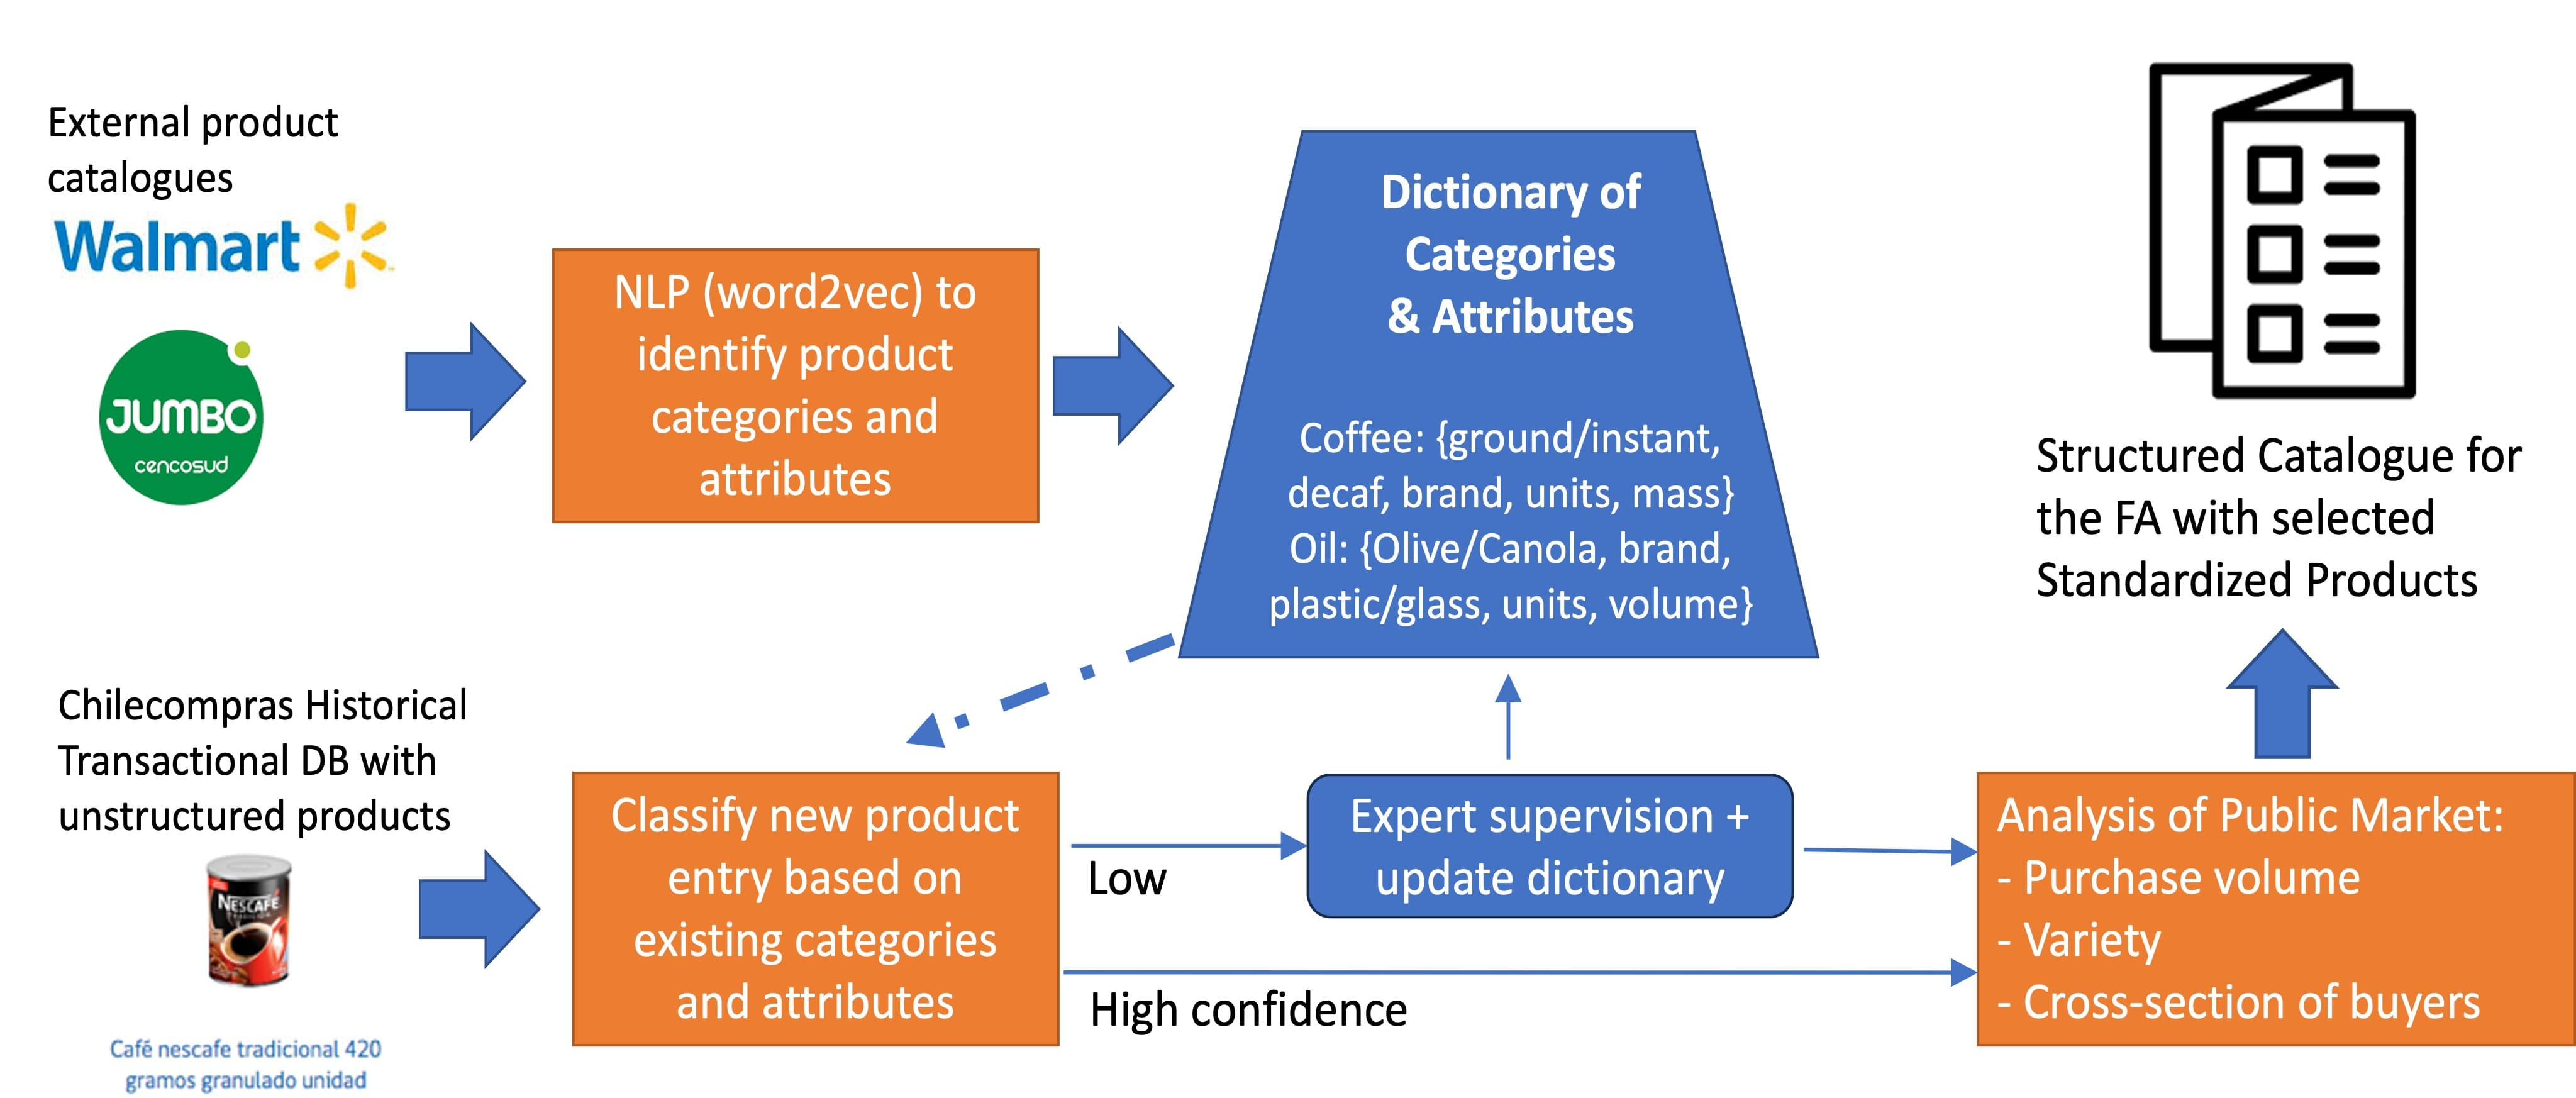
\includegraphics[scale=0.5]{imagenes/procurement/Catalogue_automation.jpg}
    \small{\textit{Notes:} Catalogues from external retailers are used to create a product dictionary, associating each category with specific attributes. A combination of Natural Language Processing algorithms are used to detect attributes for the different product categories. The trained algorithm is then used to identify attributes of products transacted in the FA 2014. This structured catalogue is analyzed to identify products (and their attributes) that are regularly purchased in the public market, which is then used to define the product catalogue for the FA 2017.}
    \label{fig:catalogue_automation}
\end{figure}

First, we collected data from external retail catalogues published online and defined a basic product hierarchy based on this catalogue. We used external catalogues because product descriptions and their categorization were more precise and consistent compared to the product descriptions of products sold in the 2014 Food FA used by ChileCompra. 

Second, we processed the unstructured text of product descriptions in the external catalogues to identify relevant attributes that could be used to standardize products. Figure~\ref{fig:NLP} illustrates this process. The classification involves two steps: (1) identifying the category corresponding to that product (i.e., pasta, coffee, soft-drinks); (2) identifying the specific attribute values that describe products in that category (brand, size, container type, units per package, among others).
The identification of attributes combines unsupervised and supervised methods. In a first pass, we used Word2Vec (\cite{mikolov2013distributed}) to identify words (tokens) that appear within a similar context in the product descriptions. For example, for soft-drinks category the tokens ``300ml",``1.5lts" and ``2000cc" appear in similar contexts in the text. Each token group is revised by a human to assign a corresponding attribute for this product category -- in this example, the tokens describe the \textit{size} attribute of the soft-drink. Because the attribute take numerical values, it is also assigned a \textit{size unit} attribute --  in this example, the values of these attribute include ``lts" (liters) and ``cc" (cubic centimeters). This process results in the definition of a dictionary that contains a set of product categories, each of them with a corresponding set of attributes and their possible values. Using unsupervised methods to process the large number of product descriptions  is essential to scale the construction of this dictionary.

As the catalogue's dictionary gets populated, the NLP algorithm can be used to predict the attributes of a product based on their {text} description, using a measure of distance of each description with those products that have already been correctly classified. These predictions are done sequentially to first detect the product's category and then values associated with each of the attributes for that category. Each prediction is associated with a confidence level, using a pre-specified threshold to decide whether the prediction required a manual (human) inspection for validation or not (see Figure~\ref{fig:NLP}). This approach consisting of hybrid classification using NLP and manual inspection was based on the work of \cite{sun2014chimera} and adapted to the context of our data (see \cite{guerra2019diseno} for details).


\begin{figure}[t]
\caption{Structure of the Natural Language Processing algorithms used to identify attributes from free-text product descriptions, combining unsupervised Machine Learning methods and manual classification}
    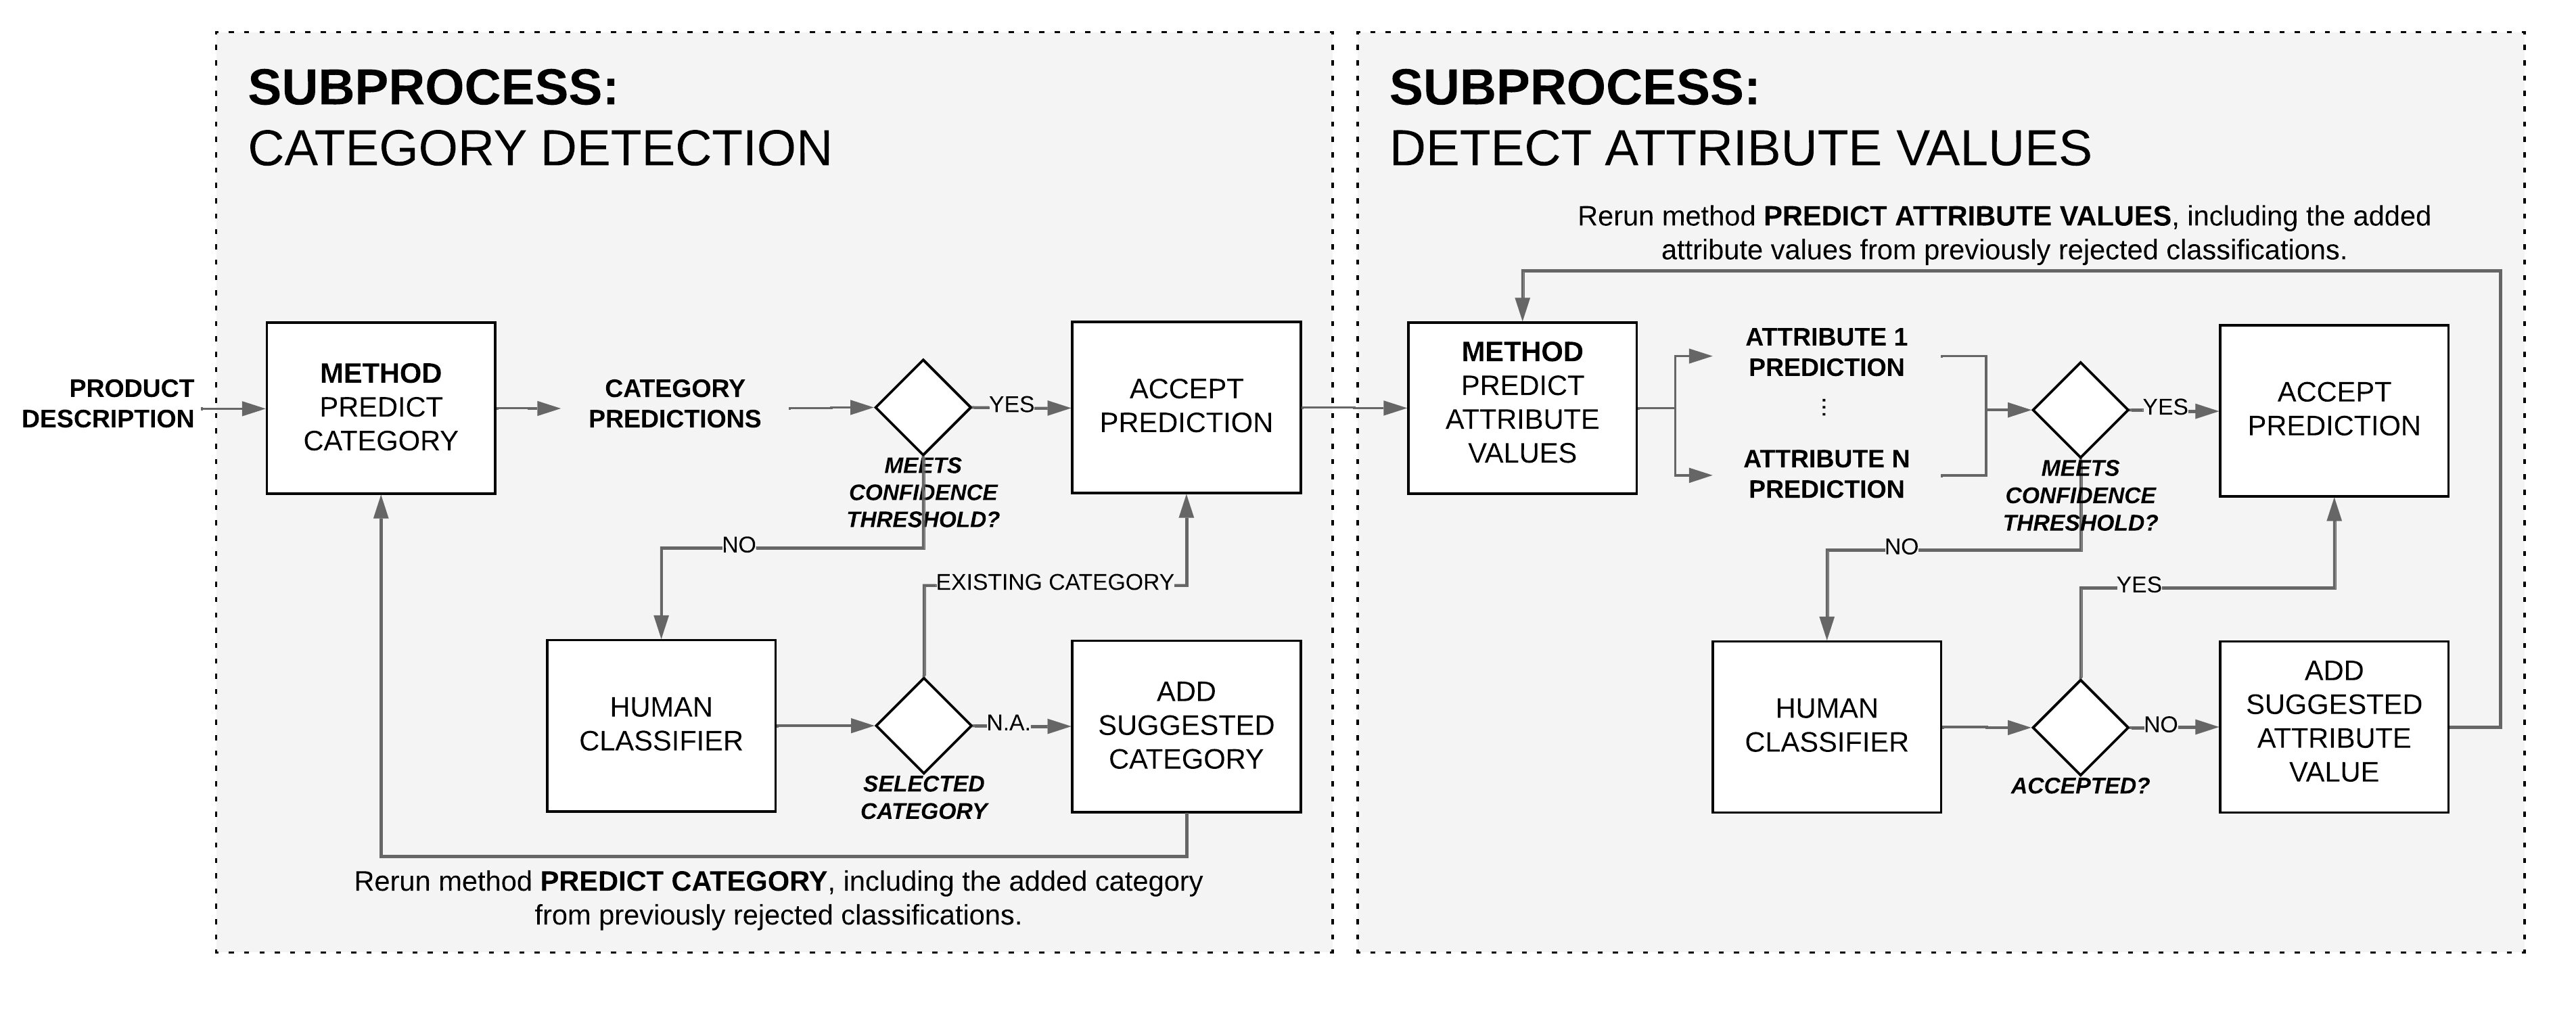
\includegraphics[scale = 0.2]{imagenes/procurement/Attribute detection.jpg}
    \small{\textit{Notes:} Unsupervised algorithms were first used to discover an initial set of product categories and attributes. Unstructured text with product description were processed sequentially using the Category Detection Method to identify the product category and then use the Detect Attribute Values method to identify the value of each attribute assigned to that category. When the predictions do not meet a minimum confidence threshold, the product was revised manually to assign a category and attributes and add the labeled classifications to the predictions. (Source: \cite{guerra2019diseno}, translated by the authors). } 
    \label{fig:NLP}
\end{figure}

As a result of this standardization, each product is uniquely defined by a set of verifiable attributes, which include \textit{category}, \textit{type}, \textit{brand}, \textit{size} and \textit{units/pkg}, plus additional attributes that vary across categories. Table \ref{tab:example_attributes} shows examples of the attributes assigned to product descriptions. \textit{Category} is a generic classification for the product, such as bottled water, canned food, or yogurt.  \textit{Type} refers to a more detailed product specification, a refinement of the  category, which is further specified by a separate \textit{brand} attribute.
The attribute \textit{size} refers to the unit of measurement of a single unit of product, that is, the number of grams (gr.) or milliliters (ml.) in the product container. Finally, products may contain a number of units per package (\textit{units/pkg}). For instance, water might be offered in individual bottles or six packs. Providing this level of detail in the units measurement was important to standardize  bids in the FA auctions.

%\newpiero{Table 2: Example of standardized products for the 2017 Food FA generated using the NLP algorithm. This table shows examples of products in the FA 2017 and their attributes (subcategory, type, brand, format and units.}

\begin{table}[H] 
\caption{\label{tab:ex_prod_2017} Example of standardized products for the 2017 Food FA generated using the NLP algorithm.}
%\centering 
 
 \resizebox{\textwidth}{!}{ 
\begin{tabular}{@{\extracolsep{5pt}} lp{6cm}lp{3cm}p{2cm}ll} 
\\[-1.8ex]
\hline \\[-1.8ex] 
\textbf{Product I.D. }& \textbf{Full Product Description} & \textbf{Subcategory} & \textbf{Type} & \textbf{Brand} & \textbf{Format} & \textbf{Units} \\ 
\hline \\[-1.8ex] 
$1477739$ & sparkling mineral water Next bottle 500 ml.~1 unit & water & sparkling mineral water & Next & 500 ml. & $1$ \\ 
$1445299$ & water-based canned salmon Robinson Crusoe bundle of 3 units 80 gr. & canned-food & water-based canned salmon & Robinson Crusoe & 80 gr. & $3$ \\ 
$1449854$ & ravioli Carozzi meat bag of 400 gr.~1 unit & pasta & ravioli & Carozzi & 400 gr. & $1$ \\ 
$1450212$ & instant coffee Nescafe can 420 gr.~1 unit & tea, coffee & instant coffee & Nescafe & 420 gr. & $1$ \\ 
$1479364$ & probiotic yogurt Uno multifruit bottle 90 ml.~12 units & yogurt & probiotic yogurt & Uno & 90 ml. & $12$ \\ 
$1443780$ &  juice Watt's nectar peach bottle 1,5 lt.~1 unit & juice  &  nectar & Watt's & 1,5 lt. & $1$ \\
\hline \\[-1.8ex] 
\end{tabular}}
 \small{\textit{Notes}: Each product description is decomposed into five attributes: subcategory, type, brand, format, and number of units. Actual product descriptions were originally in Spanish and were translated to English in this example to facilitate the interpretation of the attribute classification.} \label{tab:example_attributes}
\end{table} 

As the algorithm training process was conducted using external catalogues from private retailers, it becomes necessary to specify which of these products should be included in the final catalogue of the FA 2017 auction. This was done by identifying the actual need of these products from the buyers in the public sector, using the trained algorithms to classify the free text descriptions of the products offered in the 2014 Food FA.\footnote{Because some of the description of the products in the FA were offered by small and medium businesses, the algorithm had a lower performance in classifying this products initially. Nevertheless, predictions with low confidence were manually revised following the same procedure described in Figure \ref{fig:NLP}, thereby expanding the dictionary and improving the accuracy of the algorithm on subsequent products.}  In some cases, the algorithm identified new products purchased in the FA 2014 that had not been in the original catalog constructed from external sources.

All the information collected through this product classification was matched with transaction data in the public market to measure the volume of purchases associated with each product and their corresponding attributes. {This provided information about buyers' revealed preferences for the different products.} Moreover, hedonic price regressions (\cite{rosen1974hedonic,greenstone2017continuing}) were used to identify product attributes that were associated to high prices (e.g. specific brands), which could be associated to differences in quality. 

\textit{With all this information at hand, ChileCompra decided which products to include in the final catalogue of the new Food FA, considering adequate coverage to meet buyers' needs, incorporating different levels of product quality .}

{One potential concern of structuring the product catalogue would be a reduction in the variety of products offered in the marketplace. To that end, we analyzed the FA 2014 with the objective of assessing the product variety that was actually included in that catalogue. We focused the comparison on 9000 products of the FA 2014 which correspond to packaged food products -- referred to as \textit{pantry} -- for which it was possible to identify multiple attributes to describe them. For the remaining non-packaged food products -- meat, fresh produced, among others -- it was not possible to identify objective attributes from their description. Hence, we focused the data analysis on pantry products to assess which of these products to include in the new catalogue (for non-pantry, the product selection process was more qualitative and conducted manually by Chilecompra).}

{As expected, many of the auctions ran in the FA 2014 corresponded to products with the same attributes. Of the nearly 9000 packaged products listed in the FA 2014 (each corresponding to a separate auction), it was possible to identify attributes on 7600 of them.  This product categorization reveals that these in fact corresponded to only 2,700 unique products, based on the attributes specified for each product. {Moreover, many of these products had few transactions: the top 2000 products account for 92\% of purchases. Based on this analysis, ChileCompra opted to roughly include comparable 2000 products in the FA 2017 catalogue, which  covered most of the variety of products that were sold in the FA 2014.} 

This structured catalogue based on standardized product attributes was useful to better design the auction stage of the FA and increase competition among suppliers to enter the FA through a bidding process for {specific products}.  We describe the new auction design that leveraged the new structured catalogue in the next section.}


\subsection{Implementing changes to the FA auction rules}\label{sec:auction_rules_changes}

The new auction design incorporated several rules that can be grouped into four major changes (a summary of these changes is also presented in Table~\ref{tab:improvements}).

First, the auction stage is conducted in two phases: technical and economic evaluations. The technical phase verifies specific qualifications of the suppliers based on sales history, infrastructure, and financial statements. After passing the technical evaluation, the second phase focuses in the bid prices to define the awarded bids. This two-phase format is the standard recommended by the World Bank to increase transparency in public procurement (\cite{worldbank})

Second, the structured catalogue generated through the NLP algorithm described in the previous section defined the actual catalogue of products for the 2017 Food FA auction. This selection of products broadly covered the procurement needs of the different government units. The first  stage of the FA is designed as a set of independent auctions, {one per unique product in the catalogue} (defined by the specific verifiable attributes). In contrast to the rules used previously (including the rules of the 2014 Food FA), the new design prevented suppliers from adding new products in the auction stage.

Third, bidding rules were set so that bid prices included the product and delivery costs, with predefined minimum order sizes to reduce transportation costs for the suppliers. As distribution costs can vary significantly across different regions of Chile (urban vs.~rural areas and proximity to centralized warehouses), the country was divided into a set of geographic regions and auctions were run separately for each region for all products. This allowed suppliers to submit different bid prices for the same product across different regions, which were awarded separately.

\textit{All the previous changes were applied for all the product categories in the new FA. }

As a fourth adjustment, we changed the way in which winning bids are decided for each auction. Awarded bidders were set as a percentage of the bids submitted to each auction, with a minimum of 3 awarded bids to ensure an adequate supply. Since this was a major change in the auction rules used historically by ChileCompra, it was implemented through an experimental design  assigning different awarding thresholds for different products categories.  Recall from the discussion in Section~\ref{se:noncomp} that, a priori, it was not clear whether setting a more competitive award rule would result in lower transaction prices.  Providing empirical evidence through an experimental design was critical to measure the impact of increasing competition and inform the design of future FA auction designs. The implementation of this  experiment is described in detail in Section~\ref{sec:impact}.

\begin{table}[]
\caption{Main innovations in the design of the new Food FA.}
    \centering \small{
    \begin{tabular}{p{0.2\linewidth}|p{0.35\linewidth}p{0.35\linewidth}}

 Design attribute & Previous FA  & New FA \\
 \hline
\textbf{Initial product catalogue}
    & Few products, low standardization.  Allows suppliers to define products and add new products during the operation stage.
    & Many products in the initial catalogue. High standardization based on specific attributes, limited options to add new products during the operation stage.
    \\
    \hline

\textbf{Winner allocation}
    & Low competition to enter the FA due to low product standardization. Many auctions with single bids. {Low selectivity in awarding process.}
    & High standardization increases competition to enter the FA. {Experimental design to test different competition levels in the awarding process.}
    \\
    \hline
    
% \textbf{Price uncertainty}
%     & Slow and inaccurate price adjustments during the FA operation. High ceiling prices.
%     & Fast adjustment through time-series forecasting based on objective external market information.

\end{tabular}
} 
    \label{tab:improvements}
\end{table}

In addition to these changes in the auction design, the new Food FA included some additional innovations to facilitate the operation of the FA. A price index mechanism was introduced to reduce suppliers' exposure risk to market fluctuations. Price indexes were adjusted every six months based on external price indexes published by the government statistics bureau (Instituto Nacional de Estad\'isticas).\footnote{See \cite{gur2017framework} for a theoretical motivation of this intervention.} Second, suppliers would face restrictions to add new products during the operation of the FA. Only a limited number of new products were allowed per year, which had to be previously authorized by ChileCompra to ensure that these product were not already offered in the existing assortment.\footnote{To reduce administrative costs of Chilecompra, product descriptions where validated with the NLP algorithms in order to determine if they were already offered in the new FA catalogue.}

The auction rules were published in August 2017, followed by one week of consultations by suppliers. Technical evaluations began in November 2017; technically qualified suppliers began submitting bids starting in March 2018. Winners were awarded in June 2018 and the FA operation started in August 2018.

The auction stage included 52,844 auctions, which received on average 5.3 bids per auction, higher than the 3.4 bids per auction that were received in the 2014 Food FA auction. Recall that the 2017 Food FA auctions were run locally on each region whereas in the 2014 Food FA there were many auctions that covered the whole country; therefore, it was notable that the average number of bids per auction increased in the new FA. {This also explains the increase in the number of auctions.} Moreover, the percentage of single-bid auctions decreased from 51.2\% to 28.7\%, suggesting that the new auction design was effective in inducing more competition in the auction stage. The next section describes the methodology used to measure the impact of this new auction design on prices and procurement expenses.


% \begin{figure}[H]
% \centering
% \includegraphics[scale=1]{figures/operation_fa_img.pdf} 
% \caption{\label{fig:FA_timeline}}
% \end{figure}

\section{Measuring the impact of increasing competition in the FA auction} \label{sec:impact}

A fundamental change in the new Food FA was the construction of a structured catalogue defined by Chilecompra, which is used to define separate auctions for each product to award the suppliers that enter the FA marketplace. There was consensus among the stakeholders at Chilecompra that this new catalogue would increase efficiency in several dimensions: lowering the administrative costs of processing the bids, reducing redundancy of products and improving the organization of the catalogue in the marketplace. Hence, the standardization of the catalogue was implemented across all the product categories of the new 2017 FA.

However, there was debate on how much to intensify competition in the auction stage, {given the trade-off between reducing ceiling prices at entry and promotions in the operation stage.}\footnote{It is also common for the non-awarded suppliers to complain and file grievances on the awarding process; a more competitive entry would increase the risk in this dimension if price reductions were not significant.} 
 It therefore became critical to provide convincing evidence of the actual impact of increasing competition in the auction stage, for which \textit{we implemented the new Food FA  through a field experiment focused on measuring the effect of different levels of competition}. This approach consisted in defining two alternative awarding rules -- with high and low competition in the auction stage -- which were randomly assigned to product categories. We then compared the bids and prices of these products in the FA 2017 relative to the FA 2014,  which required matching products with similar attributes across the two FAs. This sample of matched products was used to conduct a difference-in-differences regression to measure the impact of inducing more competition in the auction stage. Note that all the products in the new FA were part of a structured catalogue, therefore the experiment focuses in measuring the \textit{incremental effect} of increasing competition in an FA were all products are defined through a standardized set of attributes. This section describes the design and implementation of this field experiment, and the econometric models used to measure its impact on bids and prices.

\subsection{Experimental design}

The implementation of the new Food FA was designed to measure the implications of increasing  competition in the auctions used to select the suppliers that enter the FA. This was conducted through an experimental design where each product auctioned in the new Food FA was assigned to one of two possible groups based on its awarding thresholds. In the \textbf{Noncompetitive (baseline) group} the lowest 80\% of all received bids in the auction were awarded and included in the FA assortment. In the \textbf{Competitive (treatment) group}, only the lowest $20\%$ of all received bids in the auction were awarded and included in the FA assortment.

In both cases, the rules imposed a minimum of three bids awarded so as to reduce potential risks in the supply (due to limited availability, delays in the distribution, among etc.). For example, if an auction in the competitive treatment received 10 bids, then the three lowest-bid products would be added to the FA, effectively awarding  30\% of the bids (not 20\%). All the other changes in the rules of the auction described in Section~\ref{sec:auction_rules_changes} were applied to \textit{all} auctions regardless of whether they were assigned to the baseline or the competitive treatment. Hence, the randomized assignment of this treatment allowed us to isolate the impact of this design variable on the outcomes of interest: inducing more competition to enter the market. 

Product categories were assigned randomly to the competitive and noncompetitive treatments. We chose to make the assignment at the product category level so as to avoid having two close-substitute products being assigned to different competitive treatments alleviating interference effects and concerns regarding {the Stable Unit Treatment Value assumption (SUTVA) required to identify a global treatment effect.} Of the 45 proposed assignments, ChileCompra changed one assignment from competitive to noncompetitive and one from noncompetitive to competitive.\footnote{Rice was moved from the competitive to the noncompetitive treatment in order to increase the likelihood of allocating to local suppliers. Coffee and Tea was moved from the noncompetitive to 
 the competitive treatment because it was considered an important category to enhance competition, given the large volume of purchases.}

 \subsection{Matching products across FAs}\label{subsec:matching}

 We sought to compare the bids and prices of products in the old and new FA, as well as of the two competitive treatments to measure the impact of the new design. {To do so, we relied on the product characterization provided through the NLP algorithms described in Section \ref{sec:standardization}. Recall that products in the old and new FA were standardized by identifying comparable product attributes from the information contained in the product description. Because some of the products changed their format across years, we generated groups of products that were ``close'' in the space of attribute values. For example, bottles of 950 ml. and 1 liter were considered to be similar in that attribute. In general, two products were associated with the same standardized product if: (i) they shared the same category, product type, brand, and format (e.g., grams); and (ii) the percentage difference between the format values was less than 20\%. }
 
 {While in principle we could apply this methodology to any product in the catalogues, in some product categories of the FA 2014 product description did not contain sufficient information to identify attributes and NLP was unable to categorize them correctly. Consequently, we focused the econometric analysis on pantry products (corresponding to packaged product categories) and excluded fresh bread, vegetables, fruits, seafood, meat products, and others perishable product categories for which the attributes detected in the FA 2014 were not sufficient to describe the product's quality.\footnote{ To be clear, these categories where included in the 2017 FA, where all the relevant product attributes describing quality and other characteristics were specified in detailed. The reason for excluding them from the econometric analysis was due to the challenge in matching these products with poor product description in the old FA.} For most pantry products, product descriptions in the FA 2014 were sufficiently detailed to identify attributes through the NLP algorithms; this selection includes 35 product categories, which comprised our initial sample for analysis.}
 
 Table \ref{tab:matching_results} shows the results of this attribute identification and matching across the two FAs. For the FA 2014, products with identified attributes---7,642 out of 8,937 products---accounted for more than 90\% of the sales of {pantry products in the FA}, which shows the high degree of effectiveness of the product standardization algorithms  {for these product categories}. Using these attributes to identify similar products, we found that these 7,642 products actually corresponded to 2,703 \textit{unique} products. Of these 2,703 unique products, 928 products had a match with a product in the 2017 Food FA (based on the criteria described above). These matched products account for about 68\% of the sales of pantry in FA 2014, and 74.1\% in the FA 2017.  These matched products defined a representative sample that was used to evaluate the impact of the changes in the FA design, by comparing the prices of the same standardized products across the old and new FAs.
 
 
 \begin{table}[H]
\centering 
\renewcommand{\TPTminimum}{\linewidth}
\small{
\begin{threeparttable}
\makebox[\linewidth]{%
%\setlength\extrarowheight{-3pt}
\begin{tabular}{@{\extracolsep{-5pt}} p{8cm}ll} 
\\\hline 
 & \multicolumn{2}{c}{No. of Products (\% sales)}\\ 
 \cline{2-3}
 & FA 2014 & FA 2017 \\ 
\hline \\[-2.5ex] 
Total number of \textit{pantry} products & 8,937 (100\%) & 3,789 (100\%) \\
Products with identified attributes & 7,642 (92.4\%) & 3,704 (97.3\%) \\
Unique products based on selected attributes & 2,703 (92.4\%) & 2,027 (97.3\%) \\
Matched products across FAs & 928 (68.2\%) & 928 (74.1\%) \\ 
\hline 
\end{tabular}}
% \begin{tablenotes}
%   \small
%      \item \textit{Note:} This table summarizes the results of the product standardization process. We say that a SKU is feasible if all the following attributes were identified: \textit{subcategory}, \textit{type}, \textit{brand} and \textit{format}. The mentioned attributes define a unique Standardized product.
%    \end{tablenotes}
\end{threeparttable}
}
\caption{Product identification summary for all \textit{pantry} products {-- packaged products which can be described through standardized attributes --} in the 2014 (old) and 2017 (new) FAs. The last row counts unique products that were found in both FAs.}
\label{tab:matching_results}
\end{table} 

 
 \subsection{Hypotheses}
 
 The main goal of inducing more competition in the auction stage is to generate lower transaction prices and thereby reduce procurement costs. There are alternative mechanisms that can lead to this price reduction. First, awarding bids to a smaller fraction of bidders---the competitive treatment condition in our experimental design---should lower the cutoff bid price, thereby leading to lower \textit{awarded bids}. Moreover, this increased competition in the auction stage might also lead suppliers to bid more aggressively, leading to lower \textit{submitted bids}, which should further reduce the awarded bid prices. Overall, we expect that auctions in the competitive treatment should have lower awarded bids relative to the noncompetitive treatment.
 
Moreover, recall that the auction stage of the FA sets the ceiling prices that suppliers can charge, but that suppliers can further lower the prices during the operation stage through price promotions. As previously discussed, while awarding a smaller number of bids may decreases ceiling prices, it is not clear that it also decreases the prices that are offered during the operation stage of the FA. Hence, 
fewer participants in the FA could potentially increase the \textit{posted} prices that suppliers set in the online platform. This increase in posted prices may also lead to higher \textit{transaction} prices at which buyers purchase these products.

Based on this discussion, we postulate the following hypotheses that we test in the next section:
 
\noindent \textit{\bf Hypothesis 1.} \textit{Lower ceiling prices}: Awarding a smaller number of bidders leads to lower awarded bids.

\noindent \textit{\bf Hypothesis 2.} \textit{Prices for the competitive treatment are lower}: {Awarding a smaller number of bidders, leads to lower posted and transaction prices.} 

 \noindent \textit{\bf Hypothesis 2 alt.} \textit{Prices for the competitive treatment are \textit{not} lower}: {Posted and transaction prices are not lower in the competitive treatment. Price competition in the FA operation may compensate for less competition in the auction.}

 
\subsection{Econometric model}

We conducted a difference-in-differences regression to measure the effect of increasing competition in the auction stage, distinguishing the alternative mechanisms discussed in the hypotheses formulation. Specifically, we sought to estimate the causal effect of the competitive treatment condition on submitted and awarded bid prices in the auction stage and posted and transaction prices during the operation stage.

\paragraph{Auction stage: Analysis of bids.}
First, we focus on studying the effect of the new FA design and the competitive treatment on the auction bids. As we explained above, bid prices correspond to the ceiling prices that the suppliers can charge during the operation of the FA. 

Let the index $t\in\{\text{Old},\text{New}\}$ represent the old (2014) and the new (2017) Food FAs, respectively.  Let $b_{ijrt}$ represent the bid offered in FA $t$ by supplier $j$ to provide product $i$ in region $r$, including shipping.\footnote{Recall that some auctions were run at the national level in  the FA 2014. However, suppliers must specify a shipping rate for all regions they seek to supply, which is used to calculate the bid price for each region.} Define $B^{med}_{irt}$ as the \textit{median} bid across all supplier bids submitted in the FA for that product-region-FA combination. In calculating this median bid price, we considered alternative methods for discarding extreme prices that could be generated by bidding mistakes or unrealistically aggressive bidding. For the main results we used a modified Tukey rule \citep{Tukey1977},\noteEL{verificar si se necesita Appendix}described in Appendix \ref{app:data}. To make the bids for the 2014 and 2017 Food FAs comparable, all prices for 2014 were adjusted using the CPI food price index. In addition, we normalized bid prices so that they represented bid prices per unit. See  Appendix \ref{app:data} for further details on data pre-processing. 

The following difference-in-differences specification is used to estimate the effect of the competitive treatment condition ---denoted by the indicator variable $Comp_{i}$--- on bid prices:
\begin{equation}
    \log (B^{med}_{irt}) = \delta_r + \gamma_i + \alpha New_{t} + \beta New_{t}\times Comp_{i} + \varepsilon_{irt} \ ,
    \label{eq:reg_sub_bid}
\end{equation}

\noindent where $New_t$ is an indicator equal to one for the new FA and $\delta_r$ is a region fixed effect. The sample is comprised of all products $i$ that were matched across the old and new FAs based on similar attributes, and the regression includes a product fixed effect $\gamma_i$. {The error term $\varepsilon_{irt}$ represents other idiosyncratic unobservable factors that affect bid prices of each product across FAs and  regions.} The coefficient $\alpha$ measures the average differences in bid prices between the old and new FAs for the noncompetitive baseline group. The key parameter of interest is $\beta$, the coefficient capturing the incremental change in bid prices for the auctions in the competitive treatment condition in the new FA.

Recall that $B^{med}_{irt}$, which is the median across all \textit{submitted} bids, measures whether the competitive treatment affects the bidding behavior of the suppliers.  Any changes in the submitted bids should carry over into the winning bids. Furthermore, the competitive treatment condition also lowers the cutoff point of the winning bids, which can lead to lower awarded bids even when submitted bids remain constant. Hence, we also estimated regression \eqref{eq:reg_sub_bid} using the median among \textit{awarded bids} as the dependent variable. Taken together, these models allow us to test Hypothesis 1, by measuring the effect of less competition in the auction stage on the winning bids and identifying what part of this reduction is due to changes in bidding behavior.



\paragraph{Operation stage: Analysis of prices.}
While the bids constitute a ceiling on the price that suppliers can charge during the operation of the FA, the ultimate goal is to reduce posted and transaction prices, which translate directly into procurement savings. To conduct this analysis, we assembled a weekly panel dataset including prices posted in the online platform and the actual transacted prices from purchasing orders. Let $p_{ijrtw}$ denote the average posted prices by supplier $j$ for product $i$ in region $r$ during calendar week $w$ in FA $t$. As with the bids, we calculated the {\em median posted price} for a product across all suppliers during that week, denoted by $P^{med}_{irtw}$. That is, $P^{med}_{irtw}$ denotes the median price at which product $i$ could be purchased in region $r$ during calendar week $w$ under the operation of FA $t$ in the period listed above. 

We estimated the panel regression:
\begin{equation}
    \log (P^{med}_{irtw})= \delta_r + \gamma_i + \tau_{wc(i)} + \alpha New_{t} + \beta New_{t}\times Comp_{i} + \varepsilon_{irtw} \ ,
    \label{eq:reg_op_posted}
\end{equation}
\noindent where $\delta_r$ and $\gamma_i$ are region and product fixed effects respectively, $\tau_{wc(i)}$ is a product category-specific calendar week dummy variable to capture potential seasonality ($c(i)$ indicates the category of product $i$). {The error term $\varepsilon_{irtw}$ represents other unobservable factors that affect prices during the operation stage.}


To analyze actual expenditures, we estimated model \eqref{eq:reg_op_posted} using as dependent variable the \emph{median transaction price} across all units that were bought during a given week. To calculate the median, we considered each unit bought as one observation. For example, an order with $n$ units for the same product is considered as $n$ different observations in the median calculation. In this way, the median considers the quantity of products sold at each price level. Notice that this panel is unbalanced because some products were not sold  every week.

Both panel regressions were estimated with data from 13 months prior to the operation of the new FA (August 2017 to August 2018) and the first 13 months of operation (September 2018 to September 2019).\footnote{Using a window of 13 months ensured that all 52 calendar weeks are considered.} Prices are adjusted for inflation according to the monthly CPI index for Food and Non-alcoholic Beverages. In addition, we eliminated outliers by applying the same procedure used for bid prices.

\subsection{Estimation results}

Table \ref{tab:main_results} shows the main estimation results showing the impact of the change in the level of competition  in the  auction stage on bids and prices. Columns (1) and (2) show the effect on submitted and awarded bids (regression \ref{eq:reg_sub_bid}); columns (3) and (4) show the effect on posted and transaction prices (regression \ref{eq:reg_op_posted}). Appendix \ref{app:robustness} contains robustness analyses and alternative regression specifications. The results obtained from these alternative regression specifications are qualitatively similar to the ones obtained with the main  specifications here.


\begin{table}[H] \centering 
\footnotesize 
\setlength\extrarowheight{-1pt}
\begin{tabular}{@{\extracolsep{-10pt}}lccp{1cm}cc} 
\toprule
 & \multicolumn{2}{c}{\textit{Bids}} & & \multicolumn{2}{c}{\textit{Prices}}\\ 
\cline{2-3} \cline{5-6} 
 & Submitted & Awarded && Posted & Transaction \\ 
& (1) & (2) && (3) & (4)\\ 
\hline
\\
 New FA & $-$0.141$^{***}$ & $-$0.055$^{***}$ & & $-$0.025$^{***}$ & 0.004$^{***}$ \\ 
  & (0.006) & (0.007) & &(0.001) & (0.002) \\
  \\
 New FA $\times$ Competitive & 0.002 & $-$0.081$^{***}$ & & $-$0.092$^{***}$ & $-$0.082$^{***}$ \\ 
 & (0.010) & (0.013) & & (0.001) & (0.002) \\ 
 \\
\hline 
Observations & 12,349 & 11,382 & & 973,195 & 180,421 \\ 
R$^{2}$ & 0.923 & 0.892 & & 0.961 & 0.974 \\ 
Adjusted R$^{2}$ & 0.920 & 0.887 & & 0.961 & 0.974 \\ 
\bottomrule
\multicolumn{5}{l}{\textit{Note:}  $^{*}$p$<$0.1; $^{**}$p$<$0.05; $^{***}$p$<$0.01} \\ 
\end{tabular} 
\caption{\label{tab:main_results} Main estimation results measuring the effect of the new FA design and the level of competition in the auction stage on bids and prices. All the specifications include product and region fixed effects. {For regressions with Bid prices, some auctions were not awarded and therefore the number of observations drops when using awarded bids (column (2)). Regressions with posted and transaction prices (columns (3) and (4)) include product category-specific calendar week dummies to control for seasonality. Since not all products are sold every week, the transaction price regressions have fewer observations relative to posted prices.} Robust standard errors for each estimated coefficient are reported in parentheses for all the models.}
\end{table} 


 The estimation results in columns (1) and (2) suggest that the baseline groups in FA 2017---which were awarded 80\% of the bids---exhibited lower bids relative to the FA 2014: the \textit{New} coefficient estimates that submitted bids were reduced by 14.1\% and awarded bids were reduced by 5.5\%. Although part of this effect may be attributed to changes in the auction design,  it is not possible to disentangle this effect from other external factors, such as changes in food prices or other fluctuations in the open market. Hence, we cannot interpret $\alpha$ as a causal effect of the new design on prices.%\todoMO{Added a line to explain the reasoning}
 
 The effect of the competitive treatment ---which was induced through a randomized experimental design--- can be interpreted as a causal effect of inducing more competition in the auction stage of the FA. The interaction term $New\times Comp$ shows that auctions that had lower thresholds for assigning winners led to lower awarded bids ---on average 8.1\% lower (column (2))--- providing support for Hypothesis 1. However, there appears to be no effect on the bids submitted by the bidders: in column (1) the coefficient of $New\times Comp$  is small and not statistically significant. This suggests that the reduction in the price of the awarded bids was not induced by changes in bidding behavior across the different auction rules (i.e., competitive or noncompetitive) but rather due to the lower awarding threshold applied in the competitive treatment group. {Note that the regressions with submitted bids include some auctions that were not awarded, hence the sample size is larger relative to the analysis with awarded bids. Appendix \ref{app:robustness} shows the estimation using the sample of awarded auctions, which yields similar results.}

In terms of prices, the results suggest that posted prices were lower across all products in the new FA design relative to FA 2014, showing a 2.5\% reduction in the price of the products in the noncompetitive treatment and an additional 9.2\% reduction of those in the competitive treatment {(see column (3) in the table)}. Overall, the reduction in posted prices of products in the noncompetitive treatment is substantially smaller than the reduction in the ceiling prices (determined by the awarded bids); that is, the pass-through from ceiling to posted price is not one-to-one. 
For the noncompetitive products, posted prices decreased by 2.5\% relative to the FA 2014, about half the 5.5\% decrease observed for the awarded bids. 

Products in the competitive treatment had posted prices that were 11.7\% lower (0.025 + 0.092) relative to the FA 2014, compared to a 13.6\% (0.055 + 0.081) drop in the awarded bid prices. One potential explanation is that in the old FA, even though ceiling prices were higher, this lack of competition in the auction stage was partially compensated for by more competition in the operation stage of the FA, as showcased by the fact that suppliers were frequently running price promotions. Overall, the new FA design combined with a more competitive auction stage was effective in reducing posted prices, and the effect is statistically and economically significant.

More importantly, the estimates on transaction prices (column (4) in Table \ref{tab:main_results}) reveal that the reduction in posted prices for the competitive treatment also translates into a significant reduction in transaction prices, in the order of 8\%, relative to the FA 2014. However, the {change} on transaction prices for the noncompetitive group is negligible. Taken together, these results provide support for Hypothesis 2: inducing more competition in the auction stage was effective in reducing posted and transaction prices, thereby lowering procurement spending for the government.  The savings in the government procurement cost amounted to US\$3.6 million  yearly if we  consider only the treatment group and to US\$11 million yearly if we extrapolate to the
entire Food FA.\footnote{The extrapolation more than doubles the savings because, as we explained before, there were many non-pantry product categories not considered in the experiment.} The results highlight the importance of introducing  a competitive entry stage to achieve reductions in procurement costs when using FA purchasing mechanisms.



\section{{Generalizing the New FA Design, Impact and Transferability}}

% \subsection{Transferability to other Framework Agreements}

 
 Through the pilot study just described, we identified important steps that were fundamental to induce competition upon entry and for the efficient operation of the FA:  product standardization and defining the catalogue of products to be procured. These steps have been adopted as part of the standard operating procedure used by ChileCompra in the design and implementation of FAs, which were formally included in the new regulation on public procurement (\cite{leycompras}). In addition, the experimental design used in the Food FA provided evidence in support of inducing more competition in the auction stage of the FAs. Based on this, ChileCompra adopted a new strategy for the design of all the FAs that were implemented after the Food FA.
 With this motivation, we collaborated with ChileCompra during August 2019--February 2020 with the objective of transferring the tools and know-how developed in the Food FA to the design of several new FAs: for office supplies, computers, office furniture, household cleaning, and hardware. This transferability was supported by a government grant, aimed at facilitating the adoption of the best practices that were identified in the Food FA pilot study.\footnote{Fondef Project ID16I10122, ``Diseño De Una Plataforma Para La Implementación De Convenios Marco Competitivos," directed by Marcelo Olivares.}

\noindent{\bf Competitive auction rules.} 
Similarly to our Food FA re-design, the new FAs had a two-stage design: a first, selection stage based on technical criteria followed by a second, competitive stage conducted through an auction based on prices. 
The design of the auction stage included a structured product catalogue, developed by ChileCompra, specifying detailed product attributes that uniquely identified the products to be auctioned. Some of these catalogues were constructed based on catalogues from the open market and processed using NLP tools (which included some extensions of those used for the Food FA). 

Moreover, the awarding rules were uniformly changed to induce more competition relative to previous FAs. 
In some of the new FAs, awarding rules were based on a fixed number of winners per auction. For example, for the Computers FA (2020), products were grouped into quality categories where the $X$ lowest bids in each quality category were awarded (the number of awardees $X$ varied between 10 and 20 across the Desktop and Laptop Computer categories, based on the potential number of suppliers). Office Furniture and Office Supplies FAs used a similar awarding criteria. For other FAs, awarding rules were defined as a percentage of the submitted bids. For example, for the Household Cleaning FA, the lowest 30\% of the received bids were awarded and  for Industrial Cleaning Products FA, where products  are bought in larger volumes, the cutoff was set at 10\%. The Hardware Products FA used similar awarding criteria.


\noindent{\bf Product standardization and product catalogue.} As discussed in Section~\ref{sec:auction_rules_changes}, to implement a competitive yet meaningful auction, it is useful to have a standardization of the products to eliminate the differentiation introduced by suppliers that would reduce the competition. The NLP methodology developed in the pilot study was further developed to improve its accuracy and packaged into a stand-alone application programming interface, funded by government grants aimed at technological transfers to the public sector. This interface was transferred to ChileCompra and made available as open source code that could be used in other public sector and non-profit applications.\footnote{The source code is available at the repository \texttt{https://github.com/rguerral/catalogador\_standalone}. }

After the implementation of the Food FA, ChileCompra changed its procurement strategy and opted to focus FAs on categories for which it was possible to describe products through observable attributes. Categories for which it was not possible to describe products through a structured catalogue (e.g., catering services, training programs) were moved from FAs to other procurement mechanisms such as auctions or direct purchases. {This led to fewer products and services being available through FAs, but these FAs exploited product standardization to generate a more competitive awarding process and thereby achieve lower prices. As a consequence of this new strategy, the share of purchases conducted through FAs was reduced from 23\% in 2018 to 11.6\% in 2021 (because there were fewer categories), but product categories operating with the new FA design were actively used by buyers.}

{\noindent{\bf Impact.}} The entire process of defining a structured product catalogue (using algorithmic NLP methods), made the design and evaluation process more efficient, thereby reducing administrative costs. The methodology for constructing standardized catalogues and introducing higher levels of competition in the FA auction stage was implemented in subsequent FAs, which in 2022 amounted to US\$800 million worth of purchases (including the Food FA).  If we were to extrapolate the treatment effect on transaction prices to these FAs, the total savings would amount to $8\% \times 800 = \textup{US}\$64$  million per year.%\todoMO{Changed the calculation}
%\subsection{Impact beyond the design of FAs}

In addition, the adoption of catalogue standardization in the design of FAs aimed at generating competition in the auction stage also enabled innovations during the evaluation and operation stage of the FA. 
First, reducing the amount of unstructured text product description enabled a more automated process for submitting and evaluating the bids. A web server was developed to receive bids from suppliers in a standard format, providing information on product attributes, prices, and other bid variables that could be used in more complex auction formats. These improvements significantly reduced the work required by suppliers to submit bids and minimize errors in the submission. This bid validation process was implemented as a stand-alone application available in open source to the public.\footnote{The source code for the bid validation interface is available in the following repository \texttt{ https://github.com/rguerral/site\_validador}. }

Furthermore, product standardization led to more structured transaction data, leading to more amenable data analysis conducted during the operation of the FA. In particular, product attributes could be used to identify groups of substitute products and compare their prices, {a key feature to develop an effective search ranking algorithm}. This was also used to develop a monitoring system to measure \textit{overspending} by government units, estimating potential savings that could be achieved by switching to substitute products with lower prices. Savings due to this monitoring system were estimated in the order of 1.5\% of expenditures, equivalent to  US\$12 million if we use the overall 2022 FA expenditures as a baseline (\cite{dipresFEI}).


\noindent{\bf Beyond ChileCompra.}
Public procurement is an important activity: among OECD countries, public procurement ranges between 20\% to 40\% of all government expenditures and between 5\% to 18\% of the countries' GDP (\cite{OECD2017_PP}). FAs are widely used across governments' central procurement agencies, and therefore, increasing efficiency of these purchasing mechanisms can have a sizeable impact on public spending. The findings of our work can be extended to any country having a central procurement agency to coordinate public purchases. Note that all OECD countries report to have a central procurement agency (\cite{OECD2015_CPB}).

In fact, some of the co-authors of this work have been advising other governments in Latin America to implement similar strategies for FAs. On a recent project (April-June 2023), we collaborated with the Ministry of Finance of Peru to evaluate the implementation of FAs, creating structured catalogues to facilitate price comparisons and generate more competition in FAs and other procurement mechanisms. We are currently in conversations with the central procurement agency of Paraguay to initiate a project that replicates the work conducted in collaboration with ChileCompra, helping them to develop a structured catalogue for FAs and designing mechanism that exploit this standardization to increase competition. In addition, through our extended collaboration with ChileCompra, we have been presenting the findings of this work to other countries and institutions (eg. OECD committees and Mexico's procurement body). We hope that these endeavors will have a real practical well impact beyond ChileCompra.

Finally, the findings also carry implications for the recent efforts in U.S. federal procurement to centralize purchasing and reduce costs, such as those outlined in the Federal Information Technology Acquisition Reform Act (FITARA).\footnote{https://www.cio.gov/policies-and-priorities/FITARA/} As procurement processes become more centralized, there is an optimal scale at which investment in technology, such as the one required to build well-structured catalogs,  becomes feasible. In such scenarios, possessing well-designed FAs, like the ones described in this work, could be a strategic choice. Different buyers within an agency can exploit the variety that a well-structured FA provides, while the centralization provided by the FA can leverage purchasing power and reduce the agency's spend.

\noindent{\bf Conclusions.} Our work shows the value of enhancing competition in FA auctions. Moreover, we provided important guidelines on how to implement FAs in practice, which have since been adopted by ChileCompra in the design of other large FAs used to purchase products and services worth US\$800 million per year. We generated decision-support tools that are now actively used by ChileCompra to improve their procurement processes beyond FAs and being considered by governments from other countries. Overall, we believe this project showcases how  market design together with machine learning can greatly improve market outcomes. 


